\documentclass[a4paper,12pt,times,numbered,print,index]{report}
\usepackage[english]{babel}
\usepackage[utf8]{inputenc}

\oddsidemargin  0.01mm       % USA 5mm?
\evensidemargin 0.01mm       % USA 5mm?
\headheight -0.03mm             % 10mm ok
\headsep  -0.03mm
\hoffset -3mm
% was commented out before
\textheight 250mm            % USA 240mm?
\textwidth 180mm             % USA 160mm?
\topmargin -10mm           % before 18/5/93 this was -20mm
\topskip -10mm

\renewcommand{\baselinestretch}{1.40}

\renewcommand {\arraystretch}{1.20}

\usepackage{dcolumn}
\usepackage{amsmath}
\usepackage{amssymb}
\usepackage{graphicx}
\usepackage{pdfpages}
\usepackage{fullpage}
\usepackage{caption}
\usepackage{float}
\usepackage{fancyhdr}
\usepackage{amsmath}
\usepackage{multirow}
\usepackage{commath}
\usepackage{natbib}
\setcitestyle{aysep={,}}
%\usepackage{apacite}
%\usepackage{biblatex}
\usepackage{mathtools}
\usepackage{subcaption}
\usepackage{mathrsfs,amssymb}
\usepackage{amsthm}
\usepackage{enumitem}
\usepackage{booktabs}
\usepackage{verbatim}
\usepackage{enumitem,kantlipsum}
\usepackage{chngcntr}
\usepackage{apptools}
\usepackage{adjustbox}
\usepackage{epstopdf}
\usepackage{pdflscape}
\usepackage{afterpage}
\usepackage[pdftex,colorlinks=true,linkcolor=cyan,linktoc=all]{hyperref}
\usepackage{siunitx}
\usepackage{authblk}
\usepackage{soul}

\usepackage{titletoc}% http://ctan.org/pkg/titletoc
\titlecontents*{chapter}% <section-type>
[0pt]% <left>
{}% <above-code>
{\bfseries\chaptername\ \thecontentslabel\quad}% <numbered-entry-format>
{}% <numberless-entry-format>
{\bfseries\hfill\contentspage}% <filler-page-format>

\usepackage[font=footnotesize,labelfont=bf]{caption}
\captionsetup[sub]{font=scriptsize,labelfont=bf}

\renewcommand{\sectionautorefname}{Section}
\renewcommand{\subsectionautorefname}{Section}
\renewcommand\thesection{\arabic{section}}

\interfootnotelinepenalty=10000
\setcitestyle{aysep={,}}
\newcolumntype{L}{@{}l@{}}
\newcommand{\mc}[1]{\multicolumn{1}{c}{#1}}
\sisetup{table-space-text-post = **}
\definecolor{darkblue}{rgb}{0,0,.6}
\hypersetup{citecolor=darkblue,linkcolor=darkblue,urlcolor=darkblue}

\makeatletter

\def\@seccntformat#1{\@ifundefined{#1@cntformat}%
	{\csname the#1\endcsname\quad}  % default
	{\csname #1@cntformat\endcsname}% enable individual control
}
\let\oldappendix\appendix %% save current definition of \appendix
\renewcommand\appendix{%
	\oldappendix
	\newcommand{\section@cntformat}{\appendixname~\thesection\quad}
}
\makeatother
\usepackage{cleveref} % just for this example

\numberwithin{equation}{section}
\newtheorem{theorem}{Theorem}[section]
\DeclareMathOperator*{\argmin}{argmin}
\newtheorem{remark}{Remark}[section]
\newtheorem{assumption}{Assumption}
\allowdisplaybreaks
\newtheorem{lemma}{Lemma}

\newcommand{\assumptionautorefname}{Assumption}
\newcommand{\lemmaautorefname}{Lemma}
\newcommand{\qedd}{\tag*{$\qed$}}

\pagestyle{fancy}
\fancyhf{}
\renewcommand{\headrulewidth}{0pt}
\cfoot{\thepage}

\title{{Parametric Single-Index Models: Simulation and Empirical Results} \vspace{2cm}}
\author{Ying Zhou}
\date{March \\ 2021}

\begin{document}
\begin{titlepage}
	\begin{center}
		\vspace*{1cm}
			
		\Huge
		\textbf{Parametric Single-Index Models: Simulation and Empirical Results}
			
		\vspace{2.5cm}
			
		\large
		\textbf{Ying Zhou} \\
			
		\vspace{0.5cm}
			
		Supervised by: \\
		Professor Jiti Gao \\
		Dr Hsein Kew
			
		\vfill
			
		A thesis presented for PhD progress review.
			
		\vspace{0.8cm}
			
		
\includegraphics[width=0.4\textwidth]{plots/monash-university-logo.png}
			
		Department of Econometrics and Business Statistics \\
			%		Monash University\\
			
		March,  2021
			
	\end{center}
\end{titlepage}
	
\pagenumbering{arabic}
	
\section{Overview}
Accurate forecasting of economic and financial variables is a challenging task in time-series analysis because the real world data have different characteristics. Simply using a transformed version of the original data (for example, taking the first order difference) may ignore some key features involved in the original data.

Linear models are the most commonly used model in economics and finance as it is simple to implement and easy to interpret. However, when integrated time-series are included, the findings concluded from linear models may suffer from potential misbalancing or spurious problem (\cite{phillips2015halbert}). Therefore, econometricians have created various models and estimation methodologies, and a vast number of studies have been published accordingly. The main objective of this thesis is to develop models and methods to deal with these problems cause by predictors with various features. 

The spurious problem occurs when variables in the regression are highly persistent. As in the study of \cite{whittington1990fertility}, which adopts a linear model to investigate the effect that tax benefits have on general fertility rate. However, since both tax benefits and general fertility rate are highly persistent, the model actually shows a misleading statistical evidence of linear relationship.\cite{crump2011fertility} revisits their study and they find no evidence of a linear co-integrating relationship between fertility and personal exemption. Thus, we considers a
semi-parametric nonlinear model with a cointegrated system. 

This model extends the fully non-parametric time-varying coefficients models developed in \cite{li2016estimation}  by adding non time-varying coefficients. This is a useful extension because it allows for the inclusion of dummy variables and deterministic time trends in the regression. We develop a multi-step estimation procedure that can be employed to estimate both the time-varying coefficients non-parametrically and the non-time-varying coefficients parametrically. We apply the proposed model to
study the impact of tax incentives on fertility. Our main findings include:

\begin{enumerate}
	\item The time-varying coefficients model suggests a nonlinear co-integrating relationship between tax benefits and general fertility rate.
	
	\item The nonlinear co-integrating relationship between tax benefits and fertility rate has weakened considerably over time.
	
	\item Even though new tax incentives have been introduced, they are not effective in increasing fertility rate any more.
\end{enumerate}

By using the semi-parametric time-varying model, we avoid the spurious problem and uncover the nonlinear co-integrating relationship between the dependent variables and independent variables. 

Another challenge in using linear predictive model is the misbalancing problem , which happens when some of the predictors have long memory and the dependent variable has short memory. (\cite{phillips2015halbert}). Stock return prediction is a typical case because stock return is stationary while most of the predictors used by previous studies are non-stationary (\cite{campbell1988dividend}, \cite{fama1990stock} and \cite{pesaran1995predictability}). In-sample, 
a large number of studies find evidence of predictability. Out-of-sample, little consensus exists on the question of whether stock return is predictable and which variables provide a better forecasting performance (\cite{welch2008comprehensive}).

To achieve a better out-of-sample performance, some researchers consider nonlinear models to capture the nonlinear relationship between stock return and its predictors (\cite{park2001nonlinear} and \cite{park2002nonstationary}). Our study extends the nonlinear model with a single integrated regressor developed in \cite{park2001nonlinear} to allow for multiple integrated regressors. The nonlinear we propose is given below:
\begin{equation}
y_{t}=f\left( x_{t-1}^{\prime }\theta _{0},\gamma _{0}\right) +e_{t},\ \ \
t=2,...,T, 
\label{NL_model}
\end{equation}
where $f\left( .,.\right) $ is a known univariate function, $x_{t-1}$ is a $d$-dimensional integrated process of order one, $\theta _{0}$ and $\gamma _{0}$ are unknown parameters and $e_{t}$ is a martingale difference process.

To help ease the curse of dimensionality associated
with estimating multivariate non-linear models with integrated time series, we present an econometric model in which the multiple integrated regressors can be reduced to a univariate single-index form via a known univariate nonlinear function. This single-index component allows for either cointegrated predictors or non-cointegrated predictors. We develop a new estimation procedure for the model. We apply the proposed model to study stock return predictability and the main findings in chapter 2 include:
\begin{enumerate}
	\item We show, via a Monte Carlo experiment, that the new estimator has
	better finite sample properties than the standard nonlinear least-squares
	estimator. 
	\item Exploiting nonlinearities in the data can lead to improved forecast accuracy relative to the historical average when predicting stock returns. 
\end{enumerate}

\textcolor{blue}{expand findings; put models in overview}

The empirical results of nonlinear models proved that by considering the nonlinear relationship among variables, the out-of-sample performance can be improved significantly. However, the nonlinear model we propose above only include integrated regressors,  while in economic and financial
studies, the regressors are a mixture of stationary and non-stationary variables. For example,  some stationary predictors are also proved to be important, such as the regression residuals in the study of \cite{lettau2001consumption}. 

In addition, the nonlinear model fail to consider the lag variables, $y_{t-1}, y_{t-2}, \cdots, y_{t-p}$, which will lead to serially correlated residuals. Therefore, we further extend model \ref{NL_model} and propose the partially nonlinear model:

\begin{equation}
	y_{t} = \beta_0^{\prime} z_t + f\left( x_{t-1}^{\prime }\theta_0; \gamma_0\right) +e_{t},\ \ \
	t=2,...,T,  
	\label{PL model}
\end{equation}%
where $z_t = (y_{t-1}, \cdots, y_{t-p}, w_{t-1}^{\prime})^{\prime}$, in which $w_{t-1}$ is a vector of stationary predictors, $g\left( .,.\right) $ is a known univariate nonlinear function, $x_{t-1}$ is a $d$-dimensional integrated process of order one, $\theta _{0}$ and $\gamma _{0}$ are unknown parameters and $e_{t}$ is a martingale
difference process.

To estimate model (\ref{PL model}), we propose a novel 3-step estimation method in which $\beta$ will have a closed form solution while $\theta$ and $\gamma$ can be estimated by the method of nonlinear least squares or constrained nonlinear least squares. As we need to use an iterative procedure to apply the nonlinear least square estimation, we choose initial values calculated from Taylor expansion to start the procedure.

The findings of this chapter are summarized as follows:

\begin{enumerate}
    \item From the Monte Carlo simulation, we find that the constrained nonlinear least square estimators have good finite sample performances
    
    \item The Taylor initial values we calculate from linear regression help further improve the performance. 
    
    \item Model (\ref{PL model}) outperforms pure linear or nonlinear models, including autoregressive models and model (\ref{NL_model}).
    
    \item The partially nonlinear model we proposed also provide a better out-of-sample performance than historical average.
\end{enumerate}

\section{Overview of the Thesis}
The thesis contains 4 chapters. The contents of each chapter are described below.
\subsection*{Chapter 1: Introduction}

The introductory chapter for the thesis reviews the relevant studies about non-stationary time series. The first part of this chapter provides an introduction to the semi-parametric nonlinear cointegration model with time-varying coefficients. The model is used to study the relationship between tax benefit and fertility rate. As the two series are non-stationary and there is a lack of cointegrating relationship (\cite{crump2011fertility}), we propose the nonlinear cointegration model to examine the instability in the time-series relationship. 

The model we propose is an extension from \cite{phillips2017estimating}. It also allows for some coefficients to be constant over time instead of being time varying because the empirical model of fertility involves two dummy variables.  We then introduce the 3-step estimation procedure used to estimate the semi-parametric model. It starts by estimating the non-parametric part and then estimates the parametric part by minimizing the sum of least squares. 

In the first part of this chapter, we will also present the empirical study results using the time-varying model. First, we uncover the nonlinear cointegrating relationship between tax benefits and fertility rate. In addition, the impact that tax benefits have on fertility rate diminishes over time. And even when new tax benefits are introduced, the diminishing impact remains the same.

The second part of this chapter introduces a parametric nonlinear model with a single-index component. This model follows the studies of \cite{dong2016estimation} and can deal with multiple non-stationary time-series. It accounts for the nonlinearities in the data and also allows for the presence of cointegrated and non-cointegrated regressors. To estimate the model, we introduce a new estimation procedure and include constraints to achieve a better finite sample performance. 

We will also present the empirical results using stock return dataset. It shows that the parametric single-index model outperforms the historical average in out-of-sample prediction. To make sure the results are significant, we apply a hypothesis test following \cite{clark2007approximately} to test the significant of the out-of-sample performances. In addition, we also follow \cite{neely2014forecasting} to produce economic utility gains relative to the historical average model. 

In the third part of the introduction, we will discuss a partially nonlinear single-index model. This model extends the parametric single-index model in chapter 2 to include lagged dependent variables and other stationary variables. We develop a 3-step procedure to estimate the model and apply truncation condition and constraint on parameters. To achieve a better convergence, we design a new method to select the initial values. We will use Monte Carlo simulation to show that the new initial values we select can significantly improve the convergence. 

The model will be applied to the stock return dataset. We can see that it has both good in-sample and out-of-sample performances. In addition, we will also discuss the out-of-sample performance of the partially nonlinear model against multiple benchmark models, such as auto-regressive model and pure nonlinear models. 

\pagebreak

\subsection*{Chapter 2: Literature Review}
This chapter provides a review of the relevant literatures on the semi-parametric time-varying model,  parametric single-index predictive models and empirical studies about fertility rate and stock return. From the review, we can see the potential challenges when use non-stationary time series. We can then discuss the importance of:
\begin{enumerate}
    \item considering a time-varying model to describe the instability in time-series relationship;
    
    \item including single-index in multi-variate time-series models;
    
    \item considering nonlinearites in financial and economic predictions;
    
    \item combining linearities and nonlinearites in empirical studies.
\end{enumerate}

\pagebreak
\subsection*{Chapter 3: Time-varying Modelling of Fertility and the Tax Benefits}
 \cite{whittington1990fertility} adopt a linear model to investigate the effect that tax benefits have on general fertility rate. They find that every increase of \$100 (in 2015 dollar) in tax benefits is associated with an increase of 2.1 to 4.2 births. However, since the variables in the regression are highly persistent, the finding may suffer from the problem of spurious regression. 
 
 \cite{crump2011fertility} revisit the analysis of \cite{whittington1990fertility} and perform a variety of cointegration tests. They find no evidence of a linear cointegrating relationship between fertility and personal exemption. This motivates us to relax the linearity assumption by allowing for instability in the cointegrating relationship.

This chapter contributes to the literature on the effect of tax benefits on fertility by estimating a nonlinear cointegrating regression model with time-varying coefficients.

\subsubsection*{Model and Methodology}
\cite{phillips2017estimating} propose the following nonlinear cointegration
model with time-varying coefficient functions:%
\begin{align*}
y_{t} &= x_{t}^{\prime }\beta _{t}+\epsilon _{t},\ \ \ t=1,...,T,
\\
x_{t} &= x_{t-1}+u_{t},  \nonumber
\end{align*}%
where $\beta _{t}=\beta \left( \tau _{t}\right) ,\tau _{t}=t/T$, and $\beta \left(
\cdot \right) $ is a $d$-dimensional vector of time-varying coefficients, $x_{t}$ is a $d$%
-dimensional $I\left( 1\right) $ processes, $u_{t}$ is a martingale difference sequence and $\epsilon _{t}$ is an error term. This is a fully nonparametric model because $\beta _{t}=\left( \beta _{1,t},...,\beta _{d,t}\right)
^{\prime }$ is an unknown function of time. 

We extend the above nonlinear cointegration model to allow for some coefficients to be constant over time instead of time-varying because
the empirical model of fertility involves two dummy variables and a time trend variable. The coefficients of these variables should not be time-varying. We therefore consider a semi-parametric nonlinear cointegration model of the form:%

\begin{equation}
	y_{t}=x_{t}^{\prime} \beta\left(\tau_{t}\right)+z_{t}^{\prime} \theta+\epsilon_{t}
	\label{tv model}
\end{equation}
where $\tau _{t}=t/T$, and $\beta \left(
\cdot \right) $ is a $d$-dimensional vector of time-varying coefficients, $x_{t}$ is a $d$%
-dimensional $I\left( 1\right) $ processes, $z_{t}$ is a $m$%
-dimensional vector containing time trend and dummy variables, $\epsilon _{t}$ is an error term.

The estimation method developed in \cite{phillips2017estimating} cannot be used to estimate a semi-parametric model because it contains a non-parametric part $\beta \left( \cdot \right) $ and a parametric part $\theta .$ Therefore, we propose a three-step estimation procedure, in which the nonparametric part is estimated first and used to construct a parametric estimator $\hat{\theta}$ in a multi-step estimation approach.

In Step 1, we rewrite model (\ref{tv model}) as follows:
\[
y_{t}-z_{t}^{\prime }\theta =x_{t}^{\prime }\beta \left( \tau \right) +\varepsilon _{t}. 
\]% 

Let $\theta $ be given at this stage and this model becomes a fully non-parametric model. Hence, we can apply the usual non-parametric estimation method and get the estimation of $\beta$:

\[
\bar{\beta}\left( \tau \right) =\bar{\beta}\left( \tau ,\theta \right). 
\]

In step 2, we estimate $\theta $ by minimising:
\[
\sum_{t=1}^{T}\left( y_{t}-z_{t}^{\prime }\theta -x_{t}^{\prime }\bar{\beta}%
\left( \tau _{t},\theta \right) \right) ^{2} 
\]%
and get the estimation of $\theta$ and denote it by $\hat{\theta}$.

In step 3, we re-estimate $\beta \left( \tau \right) $ by plugging in $\widehat{\theta}$ to define $\widehat{\beta}\left( \tau \right) =\bar{\beta}\left( \tau ,\widehat{\theta}\right)$. 

Since our model is newly proposed and we do not have the asymptotic distribution for the coefficients, we use a bootstrap method to construct the 95\% confidence interval for the time-varying regression coefficients. 

\subsubsection*{Empirical Study}
In an empirical study, we use model (\ref{tv model}) to investigate the time-varying nature of the cointegrating relationship between tax benefits and general fertility rate. Figure (\ref{chapter 1_1}) present the impact of one of the tax benefits (Subsidy) have on general fertility rate (the time-varying coefficient, blue line) along with its point-wise 95\% confidence interval (dotted lines) constructed using a wild bootstrap method.
%we follow the study of \cite{crump2011fertility} and include 3 different tax benefits: personal exemption (Subsidy), child tax credit (CTC) and earned income tax credit (EITC). We run three regressions using model (\ref{tv model}) for the three different tax benefits. models 



In the early part of the period, the impact was significantly different from zero at the 5\% level based on the
95\% confidence interval.  Beginning in the 1930s, the effect of Subsidy on the general fertility rate diminishes until the late 1940s after which they stabilize, though for most of the sample period the coefficient is statistically insignificant.

%Tax incentives used to be an effective policy instrument, but after World War II, the U.S. fertility rate is not responsive at all to tax subsidies. Overall, this study improves our understanding of how tax incentives affect people's decision to have a child.

\begin{figure}[!htp]
	\caption{Time-varying Coefficient for Subsidy}
	\centering
	\begin{subfigure}[b]{0.7\linewidth}
		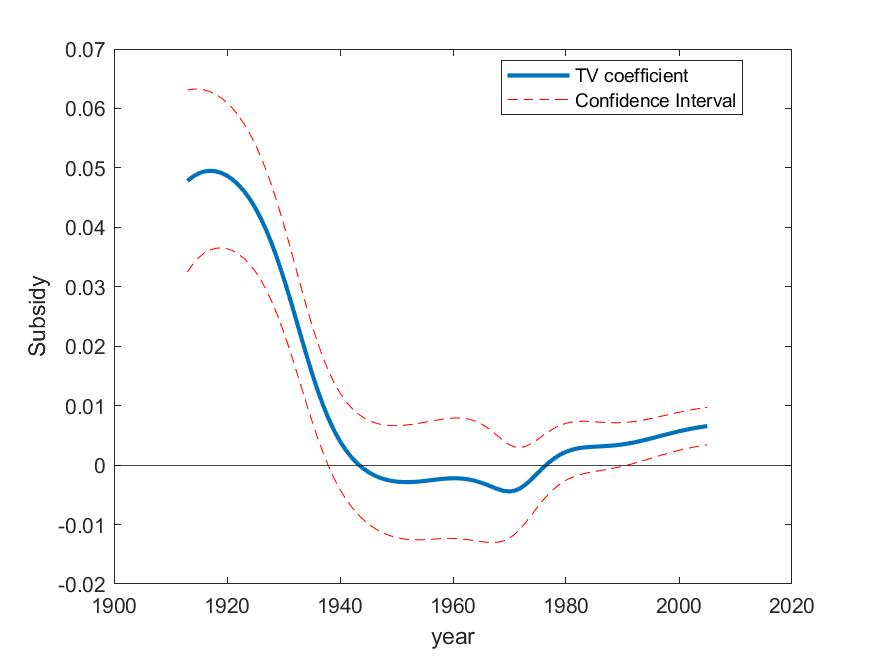
\includegraphics[width=\linewidth]{plots/CI_n201.jpg}
	\end{subfigure}
	\label{chapter 1_1}
\end{figure}

To justify that our time-varying model specifies a nonlinear cointegrating relationship between tax benefits and general fertility rate, we apply the KPSS stationarity test statistic to the residual of the regression. As the residual is stationary at 10\% level, the instability present in the cointegrating relation shown in Figure \ref{chapter 1_1} is large enough to change the conclusion of no linear cointegration. 
\begin{table}[!htp]
	\centering
	\caption{KPSS Test Results }
	\begin{tabular}{ll}
		\toprule
		& \multicolumn{1}{c}{Subsidy} \\
		\midrule
		Test Statistics & \multicolumn{1}{c}{0.0971} \\
		%        \midrule
		%        10\% Critical Value & \multicolumn{1}{c}{0.347} & \multicolumn{1}{c}{0.0885} & \multicolumn{1}{c}{0.0971} \\
		Conclusion & \multicolumn{1}{c}{Stationary} \\
		\midrule
		\multicolumn{2}{l}{\textit{\footnotesize{Note: The 10\% critical value is 0.347. }}} \\
	\end{tabular}%
	\label{tab:addlabel}%
\end{table}%
\pagebreak

\subsection*{Chapter 4: Non-stationary Parametric Single-Index Predictive Models}
Since linear predictive models fail to outperform the historical average when predicting stock returns (\cite{welch2008comprehensive}), previous studies in the empirical literature have taken nonlinearities into account when forecasting financial and macroeconomic series (see for example \cite{wooldridge1994estimation}). Following their studies, we consider a parametric single-index predictive model to forecast the stock return and investigate whether our model can achieve a better out-of-sample prediction.

%As financial and macroeconomics time-series data are usually non-stationary and cointegrated, subsequent studies have developed
%estimation methods for the nonlinear univariate econometric models with non-stationary regressors (\cite{park1999asymptotics,park2000nonstationary,park2001nonlinear}).
%
%However, when extending the univariate framework to include multivariate predictors, it suffers from the curse of dimensionality
%problem (\cite{revuz2013continuous}) because


%This model can handle a wide variety of nonlinear relationships between the regressand and the single-index component containing either
%the cointegrated predictors or the non-cointegrated predictors. 
\subsubsection*{Model and Methodology}
The nonlinear single-index predictive regression model we consider can be written as:
\begin{equation}
y_{t}=f\left( x_{t-1}^{\prime }\theta _{0},\gamma _{0}\right) +e_{t},\ \ \
t=2,...,T, 
\label{chapter_2_model}
\end{equation}
where $f\left( .,.\right) $ is a known univariate function, $x_{t-1}$ is a $d
$-dimensional integrated process of order one, $\theta _{0}$ is a $d$%
-dimensional unknown true parameter vector that lies in the parameter set $%
\Theta $, $\gamma _{0}$ is a $m$-dimensional unknown true parameter vector
that lies in the parameter set $\Gamma $ and $e_{t}$ is a martingale
difference process. The parameter sets $\Theta $ and $\Gamma $ are assumed
to be compact and convex subsets of $\mathbb{R}^{d}$ and $\mathbb{R}^{m}$
respectively.

The linear combination $x_{t-1}^{\prime }\theta _{0}$ in (\ref{chapter_2_model}) is
called the single-index component. Since $x_{t-1}$ is a vector of $I(1)$ time series, we impose the following two assumptions on the single-index component. The first assumption rules out cointegration among the predictors, $x_{t-1}$, and $\theta_{0}$ the vector of
single-index coefficients. By contrast, the second assumption permits cointegrated predictors via $x_{t-1}^{\prime }\theta _{0}\sim
I\left( 0\right) $ with $\theta _{0}$ being the cointegrating vector. 

This model: (a) accounts for the nonlinearities in the data when forecasting next period's macroeconomic and financial variables; (b) helps ease the curse of dimensionality when it comes to parametric nonlinear function estimation involving multivariate integrated regressors; and (c) allows for the presence of cointegrated regressors or non-cointegrated regressors. This model is then used to examine stock return predictability via various combinations of integrated lagged economic and financial variables.

We introduce a new estimation procedure for the model and investigate its finite-sample properties via Monte Carlo simulations. 
Model (\ref{chapter_2_model}) can be estimated by minimizing sum-of-squared-errors:

\begin{equation*}
\left( \widehat{\theta},\widehat{\gamma}\right) =\arg \min_{\theta \in \Theta
	,\gamma \in \Gamma }Q_{T}\left( \theta ,\gamma \right) .  
\end{equation*}%
where $\left( \widehat{\theta},\widehat{\gamma}\right)$ is the nonlinear least square (NLS) estimator. 

In an attempt to improve the finite sample properties of the NLS estimator, we truncate the squared-errors $\left( y_{t}-f\left(
x_{t-1}^{\prime }\theta ,\gamma \right) \right) ^{2}$ and we impose a constraint on the coefficient vector $\theta $ in the estimation procedure. To this end, we define the modified sum-of-squared-errors by%
\begin{equation}
Q_{T,M}\left( \theta ,\gamma \right) =\sum_{t=1}^{T}\left( y_{t}-f\left(
x_{t-1}^{\prime }\theta ,\gamma \right) \right) ^{2}I\left( \left\Vert
x_{t-1}\right\Vert \leq M_{T}\right) +\lambda \left( \left\Vert \theta
\right\Vert ^{2}-1\right) ,  
\label{c2_CLS}
\end{equation}%
where $I\left( .\right) $ denotes the indicator function, $%
\left\Vert .\right\Vert $ is the Euclidean norm and $M_T$ = $\sqrt{T}$. It is a positive and increasing sequence satisfying $ M_{T}\rightarrow \infty $ as $T \rightarrow \infty $ and $\lambda $ is a Lagrange
multiplier. We then obtain the constrained least squares (denoted CLS) estimator $\tilde{\theta }$ and $\tilde{\gamma}$ by minimizing (\ref{c2_CLS}).

We investigate the finite sample properties of the NLS and the proposed CLS estimators in multivariate nonstationary settings. The simulation results show that both NLS and CLS estimators have a good finite sample performance. In addition, there is significant finite sample gains from imposing the constraint on the estimation procedure when comparing the NLS estimator with the CLS estimator.

\subsubsection*{Empirical Study}
To illustrate the use of the single-index model, we provide an application to predictability of U.S. stock market returns using updated \cite{welch2008comprehensive} dataset. We find that several combinations of the predictors used in prior studies deliver out-of-sample forecasting gains relative to the standard historical average benchmark when using the single-index predictive model that accounts for the nonlinearities in the time-series data. And the hypothesis suggests that the out-of-sample predictive gain is significant at 10\% level.

In addition, we consider the realised utility gain for a mean-variance optimising investor over the out-of-sample period. Our results suggest that a risk-adverse investor who optimally allocates their resources between equities and risk-free bills can receive sizeable utility gains by using the single-index versus the historical-average forecasts.

\pagebreak

\subsection*{Chapter 5: Partially Nonlinear Single-Index Predictive Models}
In this chapter, we extend the model in chapter 2 to include stationary predictors. The new model is called partially nonlinear model. It combines linear components with a nonlinear single-index component, which can capture both linear and nonlinear relationship between dependent variable and predictors.

\subsubsection*{Model and Methodology}

In this chapter, we propose a new class of nonlinear time series models - partially nonlinear single-index models of the form:
\begin{equation}
	y_{t} = \beta_0^{\prime} z_t + f\left( x_{t-1}^{\prime }\theta_0; \gamma_0\right) +e_{t},\ \ \
	t=2,...,T,  
	\label{PL model}
\end{equation}%
where $z_t = (y_{t-1}, \cdots, y_{t-p}, w_{t-1}^{\prime})^{\prime}$, in which $w_{t-1}$ is a vector of stationary predictors, 
%such as the 3 components (consumption, labour income and asset holdings) of "cay" variable constructed by \textcolor[rgb]{ 0,  .439,  .753}{Lettau and Ludvigson (2001)}.
$g\left( .,.\right) $ is a known univariate nonlinear function, $x_{t-1}$ is a $d$-dimensional integrated process of order one, $\theta _{0}$ is a $d$-dimensional unknown true parameter vector that lies in the parameter set $\Theta $, $\gamma _{0}$ is a $m$-dimensional unknown true parameter vector that lies in the parameter set $\Gamma $ and $e_{t}$ is a martingale
difference process. The parameter sets $\Theta $ and $\Gamma $ are assumed to be compact and convex subsets of $\mathbb{R}^{d}$ and $\mathbb{R}^{m}$ respectively. In order to ensure that $\theta_0$ is uniquely identifiable, we will need to impose $\theta_{0}^{\prime}\theta_{0} = 1$. 

To estimate the model, we introduce a novel 3-step approach for estimation in order to reduce the computational burden. 

\textbf{Step 1:} set $\frac{\partial L(\beta, \theta, \gamma)}{\partial \beta} = 0$ and solve the first equation in (\ref{gradient}) to obtain $\tilde{\beta}$:
\begin{equation}
\tilde{\beta} = \left( \sum_{t=1}^{T}z_t z_t^{\prime}\right)^{-1}\sum_{t=1}^{T}\left( y_t - f\left( x_{t-1}^{\prime }\theta; \gamma\right)\right) z_t
\label{beta}
\end{equation}

In other words, $\tilde{\beta}$ is of a linear from by OLS expression. Thus model (\ref{PL model}) can be approximated by:
$$
y_t = \tilde{\beta}^{\prime} z_t + f\left( x_{t-1}^{\prime }\theta; \gamma\right) +e_{t},
$$
Substitute $\bar{\beta}$ in (\ref{beta}) and rearrange the equation above, we can get:
$$
y_t - \left( \left( \sum_{t=1}^{T}z_t z_t^{\prime}\right)^{-1} \sum_{t=1}^{T}y_t z_t \right) ^{\prime} z_t = f\left( x_{t-1}^{\prime }\theta; \gamma\right) - z_t^{\prime} \left( \sum_{t=1}^{T}z_t z_t^{\prime}\right)^{-1} \sum_{t=1}^{T} f\left( x_{t-1}^{\prime }\theta; \gamma\right) z_t + e_t.
$$

Let  
$$\tilde{y} = y_t -  z_t^{\prime}  \left( \sum_{t=1}^{T}z_t z_t^{\prime}\right)^{-1} \sum_{t=1}^{T}y_t z_t, $$ 

$$\tilde{g} ( x_{t-1}^{\prime }\theta; \gamma) = f\left( x_{t-1}^{\prime }\theta; \gamma\right) - z_t^{\prime} \left( \sum_{t=1}^{T}z_t z_t^{\prime}\right)^{-1} \sum_{t=1}^{T} f\left( x_{t-1}^{\prime }\theta; \gamma\right) z_t$$ 
Then we have an approximate model of the form:
\begin{equation}
\tilde{y} = \tilde{g}\left( x_{t-1}^{\prime }\theta; \gamma\right) + e_t.
\label{trans_model}
\end{equation}

\textbf{Step 2: } estimate $(\hat{\theta}, \hat{\gamma})$ using nonlinear least square(NLS) method. Define the sum of least squares $Q_{T}(\theta, \gamma)$ as:
$$
Q_{T}(\theta, \gamma)=\sum_{t=1}^{T}\left(\tilde{y_{t}}-\tilde{g}\left(x_{t-1}^{\prime} \theta, \gamma\right)\right)^{2}
$$
over $(\theta, \gamma) \in (\Theta, \Gamma)$.
The estimated $(\hat{\theta}, \hat{\gamma})$ is given by:
\begin{equation*}
\left( \widehat{\theta},\widehat{\gamma}\right) =\arg \min_{\theta \in \Theta
	,\gamma \in \Gamma }Q_{T}\left( \theta ,\gamma \right),  \label{nls_c3}
\end{equation*}%
which can be solved using an iterative procedure since there is no closed form solutions. 

\textbf{Step 3: } As $\hat{\theta}$ and $\hat{\gamma}$ have been estimated, we can substitute them back to (\ref{beta}) and get the estimate of $\beta$:
$$
 \hat{\beta} = \left( \sum_{t=1}^{T}z_t z_t^{\prime}\right)^{-1}\sum_{t=1}^{T}\left( y_t- f\left( x_{t-1}^{\prime }\hat{\theta}; \hat{\gamma}\right)\right) z_t.
$$.

In the 3-step procedure above, we have obtained the NLS estimators ($\widehat{\theta}, \widehat{\gamma}, \widehat{\beta}$). In order to improve finite sample properties of the estimators, we impose a truncation condition $I\left(\left\|x_{t-1}\right\| \leq M_T\right)$ on $x_{t-1}$ and an identification condition on coefficient vector $\theta$. We then define the modified sum-of-squared errors by:

\begin{equation}
	Q_{T, M}(\theta, \gamma)=\sum_{t=1}^{T}\left(y_{t}-f\left(x_{t-1}^{\prime} \theta, \gamma\right)\right)^{2} I\left(\left\|x_{t-1}\right\| \leq M_{T}\right)+\lambda\left(\|\theta\|^{2}-1\right),
	\label{CLS}
\end{equation}
where $I\left( .\right) $ denotes the indicator function, $\lambda $ is a Lagrange
multiplier and $\left\Vert .\right\Vert $ is the Euclidean norm. In equation (\ref{CLS}), the truncation condition $I\left(\left\|x_{t-1}\right\| \leq M_{T}\right)$ discards observations whose Euclidean norm is bigger than $M_T$. Similar condition has been considered by \cite{li2016estimation} and \cite{ling2007self}. $M_T$ is a positive and increasing sequence satisfying $ M_{T}\rightarrow \infty $ as $T \rightarrow \infty $. Following \cite{li2016estimation}, we choose $M_T$ = $C_{\alpha}n^{1-\beta}$ with $\beta = 1/2$ and $C_{\alpha} = 1$. Therefore, $M_T = \sqrt{T}$ in our study.    

Then we can start with step 1 above to rearrange the equations and the constrained least squares (denoted CLS) estimators $\bar{\theta}$ and $%
\bar{\gamma}$ can be obtained by minimizing $Q_{T,M}\left( \theta ,\gamma \right) 
$ over $\theta \in \Theta $ and $\gamma \in \Gamma $ such that the
two restrictions hold; that is:%
\begin{equation*}
\left( \bar{\theta},\bar{\gamma}\right) =\arg \min_{\theta \in \Theta
	,\gamma \in \Gamma ,\left\Vert \theta \right\Vert ^{2}=1}Q_{T,M}\left(
\theta ,\gamma \right) .  \label{cls_c3}
\end{equation*}%

And the CLS estimator of $\beta$ can be written as:
$$
\bar{\beta} = \left( \sum_{t=1}^{T}z_t z_t^{\prime}\right)^{-1}\sum_{t=1}^{T}\left( y_t- f\left( x_{t-1}^{\prime }\bar{\theta}; \bar{\gamma}\right)\right) z_t.
$$.

\subsection*{Monte Carlo Simulation}
We investigate the finite sample properties of the NLS and the proposed CLS estimators
for partially nonlinear model in multivariate co-integrated and non-cointegrated settings. In order to achieve better convergence, we design a unique procedure to find initial values for nonlinear least square estimation. 

From the simulation results, we find that:
\begin{enumerate}
    \item The Taylor initial values can help improve the finite sample performances of the estimators.
    
    \item Both the NLS and CLS estimators converge when sample size increases. But the constrained least square method tend to give better convergence in most cases.
    
    \item The CLS consistently perform better than the normal NLS for most functional forms. This implies that the constraint and truncation condition we proposed in section 2 do help improve the finite sample performances. 
    
    \item Among models with the 7 different functional forms, the one with polynomial functional form tend to provide the best results, but models with the two exponential functions do not perform as well as other ones.
    
    \item Models using cointegrated $x_t$ have a better finite sample performance than using the non-cointegrated $x_t$.
\end{enumerate}

\subsection*{Empirical Study}

We apply the model to the \cite{welch2008comprehensive} dataset and investigate the predictability using co-integrated variable combinations. We find that the partially nonlinear models can outperform sample mean model both in-sample and out-of-sample. When using other benchmark models, such as AR(1) model and AR(2) model, our models also provides better in-sample performance for certain variable combinations and nonlinear functional forms. In terms of out-of-sample, our models outperforms the two time series models in a consecutive period. 

And by including lagged dependent variable and the stationary "cay" variable, the partially nonlinear models give better out-of-sample forecast than the nonlinear models over a consecutive period. Therefore, we can conclude that by considering nonlinearities and auto-correlation in the dependent variable, we can achieve out-of-sample forecasting gains.

\pagebreak

\subsection*{Chapter 6: Conclusion}
The final chapter of my thesis will contain all the concluding remarks and possible future extensions.
\pagebreak

\section{Timetable}
\subsection{Statement of Progress}
Most of the materials for chapter 1 and 2 are already included in the separated chapters and papers. I will need to reorganize the materials I have and chapter 1 and 2 can be completed within a month. Chapter 3 and 4 are practically completed. For chapter 5, the simulations and out-of-sample prediction has been completed, we will need to add significance test results and the realised utility gains. This can also be finished in one month. The concluding chapter will be completed at the end.  

\subsection{Timetable}
\subsubsection{March 2022 - June 2022}
\begin{itemize}
    \item Test the significance of $R^{2}_{OOS}$ in the empirical study following \cite{clark2007approximately}.
    \item Calculate the realised utility gain following \cite{campbell2008predicting} and \cite{neely2014forecasting}.
    \item Completing Chapter 5 on the partially nonlinear model.
\end{itemize}
\subsubsection {July 2022 - August 2022}
\begin{itemize}
    \item Completing the introduction, literature review, and conclusion chapters and submit the thesis.
\end{itemize}

\subsection{Difficulties}


{\footnotesize
	\bibliographystyle{agsm}
	\bibliography{reference}
}
	
\end{document} 